%!TEX program = xelatex
% 导言区
\documentclass[12pt, letterpaper]{article}
% 文档区
\usepackage{caption}	% 可以设置脚注的各种性质
\usepackage{graphicx}	% 使用图片
\usepackage{subfigure}	% 使用子图
\usepackage{wrapfig}	% 使用嵌入的图片
\usepackage{color}	% 字体颜色
\usepackage{xcolor}
\usepackage{fullpage}	% 顾名思义
\usepackage{ctex}	% 中文支持
\usepackage{ulem}	% 字体删除线
\usepackage{amsmath}	% 公式换行
\usepackage[colorlinks,linkcolor=blue]{hyperref}	% 插入超链接
\usepackage{mathrsfs}  	% 花体


\title{判别函数}

% 正文区
\begin{document}
% 标题
\maketitle
% 目录
\tableofcontents
\newpage
本章开始为常虹讲课,英文PPT,单独看PPT无法获取到很多信息,且PPT质量一般。本文结合上课PPT与《机器学习》(周志华)进行总结。

本主要分为两部分:一、模型评估与选择;二、统计机器学习初步。


\section{经验误差与过拟合:一些基本概念}
\begin{enumerate}
\item \textbf{错误率error rate}:在一个数据集(测试集)中,分类错误的样本数占总样本数的比例。
\item \textbf{精度accuracy}:$accuracy=1-error$,即在一个数据集(测试集)中,分类正确的样本数占总样本书的比例。
\item \textbf{误差error}:1. 和2. 都是”率“。误差指的是在模型的实际输出和真实标签之间的差异,称为误差。\textbf{这个差异有很多种量化方法}。
\item \textbf{训练误差training error/经验误差empirical error}:模型在训练集上的误差称为“训练误差”(training error),也称为经验误差(empirical error)。
\item \textbf{泛化误差}:模型训练完成后,在一个新的数据集上的误差称为“泛化误差”(generalization error)
\item 
\textbf{学习的目的}:学习到所有潜在样本(包括训练样本和其他没有被用于训练的样本)普遍规律。
\item \textbf{泛化误差和过拟合}:
训练误差可以做到尽可能的小,但并不是越小越好。
我们要保证训练误差和泛化误差都尽可能的小,这样我们是学习到了尽可能多的“普遍规律”,而成功舍弃了训练集特有的特征。

训练集的一般性质没有学好的情况称为欠拟合。学习过了头,把训练集特有的性质给学了(\textbf{还不一定学到了一般性质}),称为过拟合。
欠拟合更加容易解决,过拟合是机器学习面临的关键障碍,每一类学习算法必然带有一些针对过拟合的措施。但是也要意识到,只想相信$P\leq NP$,那么过拟合就是无法避免的,所能做的就是减少其风险。
\end{enumerate}

\section{评估方法和测试误差}
为了对泛化误差进行评估,我们通常需要一个“测试集(testing set)”来测试学习器对新样本的判别能力,然后以测试机上的“测试误差(testing error)“作为泛化误差的近似。

显然,测试集和训练集应该是互斥的。测试集理想情况下应该是从样本的真实分布中独立同分布采样获得。下面是获取实际情况中获取训练集的一些方法:

\subsection{留出法}
直接把数据集$\mathcal{D}$划分成两个互斥的集合,其中一个作为训练集$\mathcal{S}$一个作为测试集$\mathcal{T}$。这种方法很直白和常用,但是要注意训练/测试数据集合的分布保持一致。另一个需要注意的问题是,即便是保证了训练/测试数据集保持一致,但是也会有多种划分方法。因此,单次留出法得到的估计结果往往不稳定。一般要采用多次随机划分,重复实验评估后取平均值作为结果。

例如进行100次划分,每次都会产是一个训练/测试数据集,每次都会产生新的结果。把最后的这100个结果作为平均就是留出法最终的结果。

一般来说,将数据集的2/3 -- 4/5用于训练,剩余的用于测试。
\subsection{交叉验证法}

\subsection{自助法}

\subsection{调参和最终模型}


\section{性能度量}



\section{偏差与方差的概念}
\subsection{以变量的视角去看训练过程}

首先要明确一点的是,方差和偏差的概念是针对泛化能力来说的。

事情可以这样理解。假如我想要根据一些输入信息预测一些输出信息。例如预测房价变化吧,最理想的情况下,我应该需要取到所有可能的数据,然后用于训练,训练结果的一般性就最会最强。但是这个“所有可能的数据”一般是无穷无尽的,无限数量的,显然是不可能做到这一点的。我们只能拥有一部分的数据集,称为训练集$\mathcal{D}$。

下面开始训练,于是我们选定了一个模型,然后用这个训练集去训练。训练得到了一个结果$f(\mathbf{x;\mathcal{D}})$。既然训练集是“所有可能的数据”的一部分,那么这个训练结果也不会对应所有数据产生的训练结果。随着选取的数据集的不同,这个训练结果是不同的。

即数据集$\mathcal{D}$是一个变量,其输出$f$自然也是一个变量。但是有一点,这所有的训练结果的平均应该是接近哪个“所有可能数据“的输出结果的(假如所选的数据集足够多且大的话)。
假设训练结果f的期望为:
$$
\bar{f} = E[f]
$$

训练结果f的方差为:
$$
\sigma_f = E[(f-\bar{f})^2] = var(\mathbf{x})
$$

\subsection{泛化误差的期望}

该模型函数$\bar{f}$的输出和真实标签之间的差距,就是这个模型的误差,也是这个模型和理想中的函数之间的偏差Bias:
$$
Bias^2(\mathbf{x}) = (f(\mathbf{x}) - y)^2
$$
其中,$y$是真实的、正确的标签。而数据集中的标签为$y_D$,它不一定和真实标签$y$相同,他们之间的差异,称之为噪声,是数据集的好坏产生的误差。

由于我们只能取到一部分数据,假如能够去到无数多的一部分数据,就可以得到这个噪声的大小就可以写成:
$$
\varepsilon^2=E_D[(y_d-y)^2]
$$
虽然很不幸我们的训练数据大多数情况下只有一个数据集$\mathcal{D}$,但是我们还是希望训练出来的这个模型的用在其他数据上的时候仍然一样有效。当把这个算法应用在其他数据集上,带来的误差error就称为泛化误差。

我们可以求泛化误差的期望:
\begin{equation}
\label{a}
\begin{aligned}
E(f;D)&=E_D[(f(x;D)-y_D)^2]
\end{aligned}
\end{equation}

\subsection{求解泛化误差的期望}
\ref{a}式可以写成:

$$
\begin{aligned}
E(f;D)&=E_D[(f(x;D)-y_D)^2]\\
&=E[(f-\bar{f}+\bar{f}-y_D)^2]\\
&=E[(f-\bar{f})^2] +E[(\bar{f}-y_D)^2] +E[2(f-\bar{f})(\bar{f}-y_D)]
\end{aligned}
$$

$\bar{f}$相当于是常数,由于$f-\bar{f}$和$\bar{f}-y_D$是独立的,所以有:
$$
\begin{aligned}
E[2(f-\bar{f})(\bar{f}-y_D)]&=2E[(\bar{f}-y_D)]E[(f-\bar{f})]\\
&=2E[(\bar{f}-y_D)](E(f)-\bar{f})\\
&=2E[(\bar{f}-y_D)](\bar{f}-\bar{f})\\
&=0
\end{aligned}
$$
所以,有\ref{a}又可以写为:
$$
\begin{aligned}
E(f;D)&=E[(f-\bar{f})^2]+E[(\bar{f}-y_D)^2]\\
&=E[(f-\bar{f})^2]+E[(\bar{f}-y+y-y_D)^2]\\
&=E[(f-\bar{f})^2]+E[(\bar{f}-f)^2]+E[(y-y_D)^2]+E[2(\bar{f}-y)(y-y_D)]
\end{aligned}
$$
假设噪声的期望$E_D[y_D-y]=0$,那么上式又可以写成:
$$
\begin{aligned}
E(f;D)&=E[(f-\bar{f})^2]+E[(\bar{f}-y)^2]+E[(y-y_D)^2]+E[2(\bar{f}-f)(y-y_D)]\\
&=E[(f-\bar{f})^2]+(\bar{f}-y)^2+E[(y-y_D)^2]\\
&=var(\mathbf{x})+bias(\mathbf{x})+\varepsilon^2
\end{aligned}
$$
即:
\begin{equation}
E(f;D)=var(\mathbf{x})+bias^2(\mathbf{x})+\varepsilon^2
\end{equation}
以上的$f$均为$f(\mathbf{x};D)$的缩写,期望符号$E$是使用不同的训练集得到结果的期望$E_D$的缩写。

\subsection{解释泛化误差的期望}
首先,上式是泛化误差的\textbf{期望}。这表明一个模型的泛化误差的期望来自于他的偏差、方差和数据集的噪声。(模型对应泛化误差的期望,不要搞混了泛化误差和泛化误差的期望)下面我们将分别解释三个量的定性含义:
\begin{itemize}
\item \textbf{偏差}度量了学习算法的期望预测和真实结果之间的偏离程度。
\item\textbf{方差}度量了同样大小的训练集的变动所导致的学习性能的变化,即刻画了数据扰动所带来的影响。
\item \textbf{噪声}表达了当前任务上任何学习算法所能达到的期望泛化误差的下界,表明了这个指定数据集下的机器学习问题问题的难度。
\end{itemize}

我们当然希望这三者越小越好,最好三个都是0,这样我们模型训练得到的模型总会是理想中的那个function。

\subsection{偏差-方差窘境}
任何函数都可以用连续的级数和展开,随着级数的幂次增高,函数再逐渐变得复杂。这可以作为研究的一个例子。

对于一个一次函数,显然他无法拟合多少函数。假如选定一个一次函数为模型,它所能产生的Function Set非常有限。他的函数空间非常小(非常集中),且在大多数情况下都偏离真实的函数(除非这个样本集的规律本来就是线性的)。即,一次函数作为一个简单的模型,它的方差小而偏差很大,甚至无法包含真实的函数。

对于一个非常复杂的高幂次多项式,他的拟合能力非常强,函数空间很大(但是也会变得分散),能够尽可能的接近真实的函数。但是对于每一次拟合的结果(假如使用不一样的数据),由于其拟合能力过强,可能会导致结果差距非常大。即,高幂次多项式作为一种复杂模型,他的方差大而偏差小,更可能可以包含真实的函数。


\begin{wrapfigure}{l}{7cm}
\centering
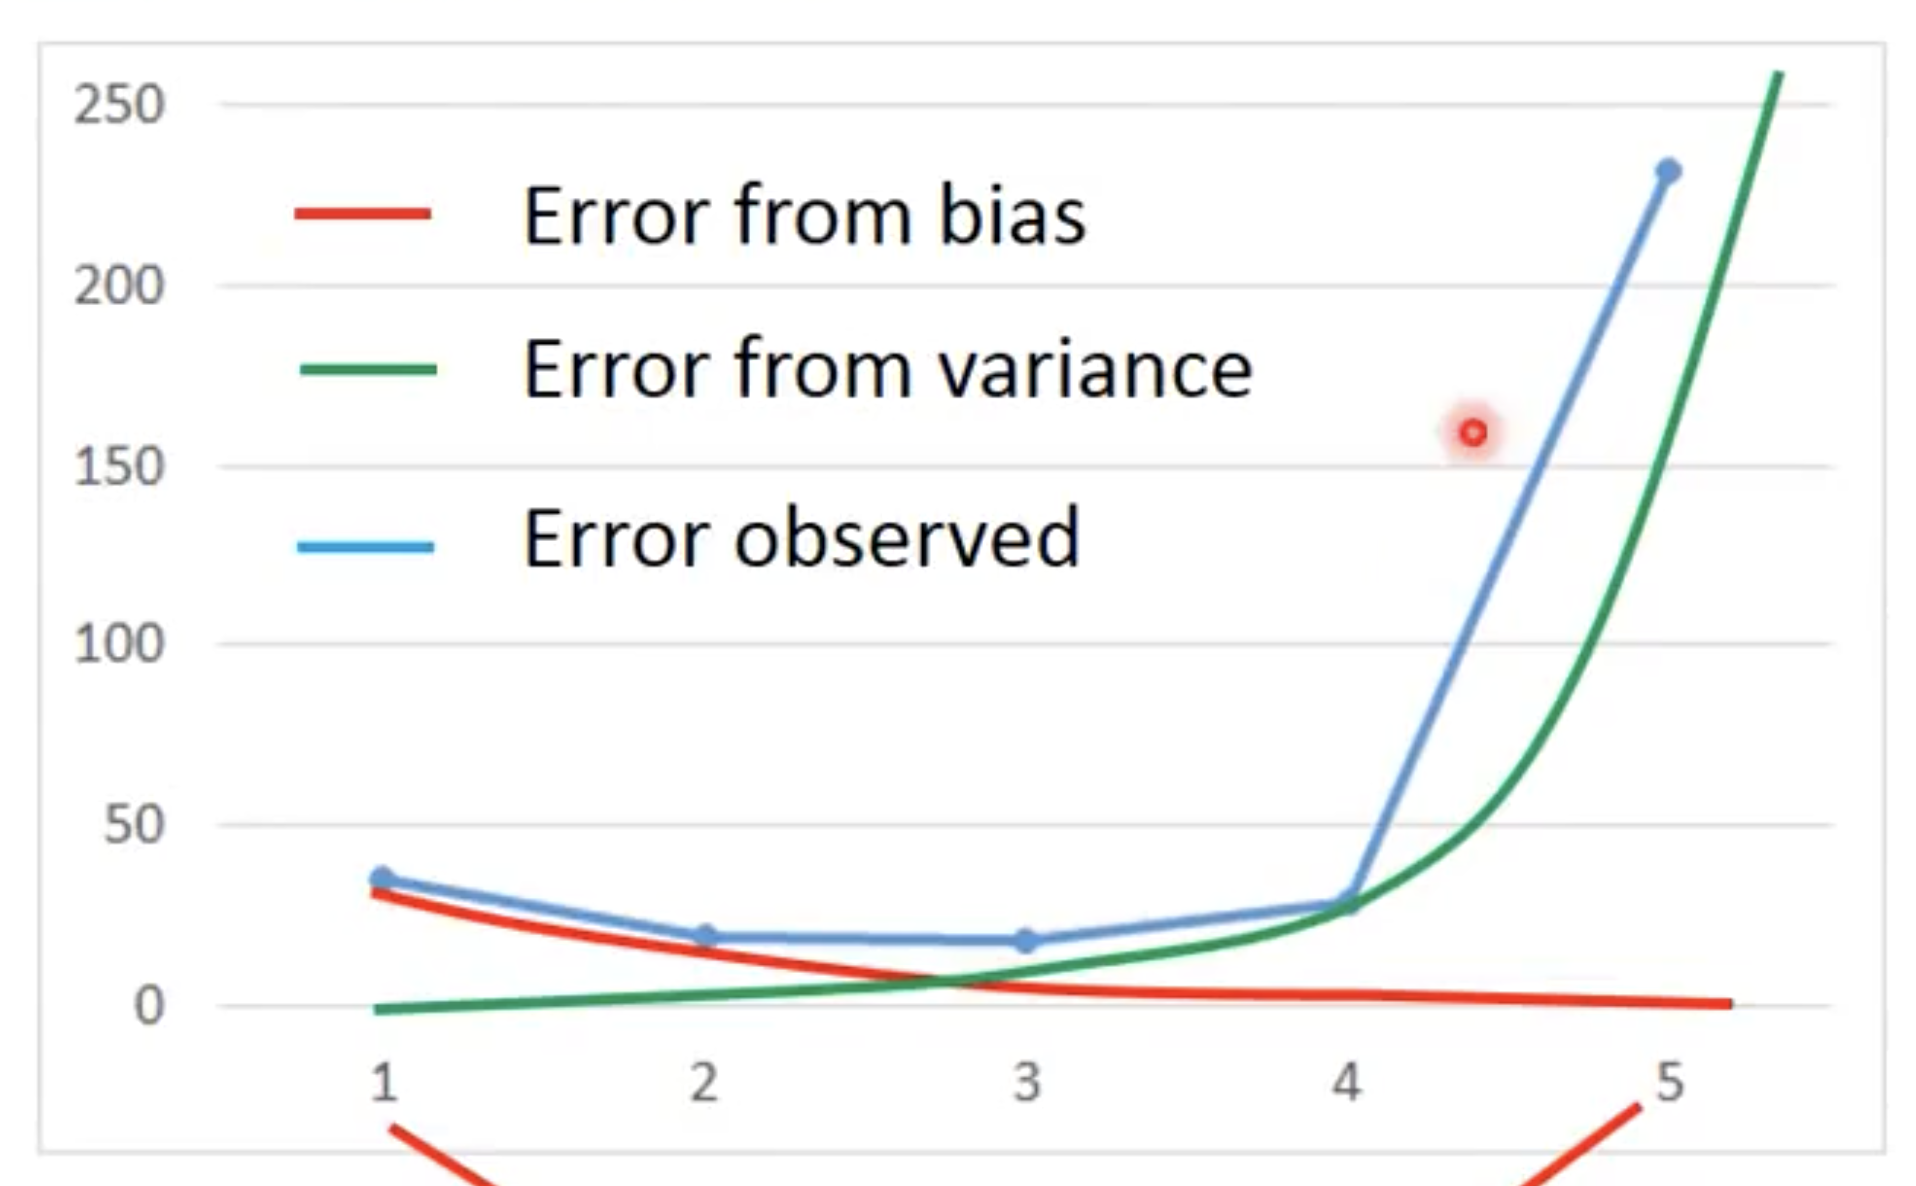
\includegraphics[scale=0.2]{BV.png}
\captionsetup{font={footnotesize}} 
\caption{训练过程中的误差和偏差的变化}
\end{wrapfigure}

对于一次函数,不需要担心过拟合的问题,因为甚至连拟合的机会都没有。对于高次多项式,只要让高次项的系数为0就可以构造出低次项的情况,但是很可能会过拟合。

再例如,使用神经网络进行训练时,开始是欠拟合的——可以理解为高次幂都还是0,随着训练的进行,复杂的部分逐渐被激活,偏差开始极大的减小,虽然方差开始增大但是总体会减小。随着训练过度进行,这个模型的偏差以及足够小了,但是由于在变得更加复杂,方差会变大,会导致泛化能力变得很差。

具体表现为,虽然在训练集上的error很低,但是当使用验证集测试其泛化能力时就会发现,泛化误差非常高。


\subsection{关于偏差和方差的更多讨论}
\subsubsection*{模型复杂度的视角}
\begin{itemize}
\item 非常灵活的模型意味着低偏差、高方差
\item 相对不不灵活的模型意味着高偏差、低方差
\item 在偏差和方差之间取得最好平衡的那些模型,是具有最好预测能力的模型。
\end{itemize}
\subsubsection*{实际价值}
知晓这个理论可能没有什么实际的价值:
\begin{itemize}
\item $\bar{f}$需要知晓所有的$\mathbf{x}$和$y$的分布,这显然是不可能的。
\item 这个理论又依赖于整体数据,但是在实际中我们只有一组数据集。
\item 但是这个理论可以让我们更好的理解训练的过程。
\end{itemize}
\subsection{Bayesian model selection}
\href{http://alumni.media.mit.edu/~tpminka/statlearn/demo/}{这里没懂}


\section{一种缓解过拟合的方法——正则化}
\subsection{简单复习线性回归Linear Regression}
\subsubsection*{线性回归的定义}
多特征的Linear Regression的表达式为:
$$
\begin{aligned}
y &= \mathbf{w^T}x\\
&=h_{\mathbf{w}}(x)
\end{aligned}
$$

其中,$\mathbf{w}$就是要求解的参数,一般也会被写作$\mathbf{\theta}$。此时的损失函数可以写为最小二乘损失(\color{red}为什么这么写?):\color{black}

\begin{wrapfigure}{l}{6cm}
\centering
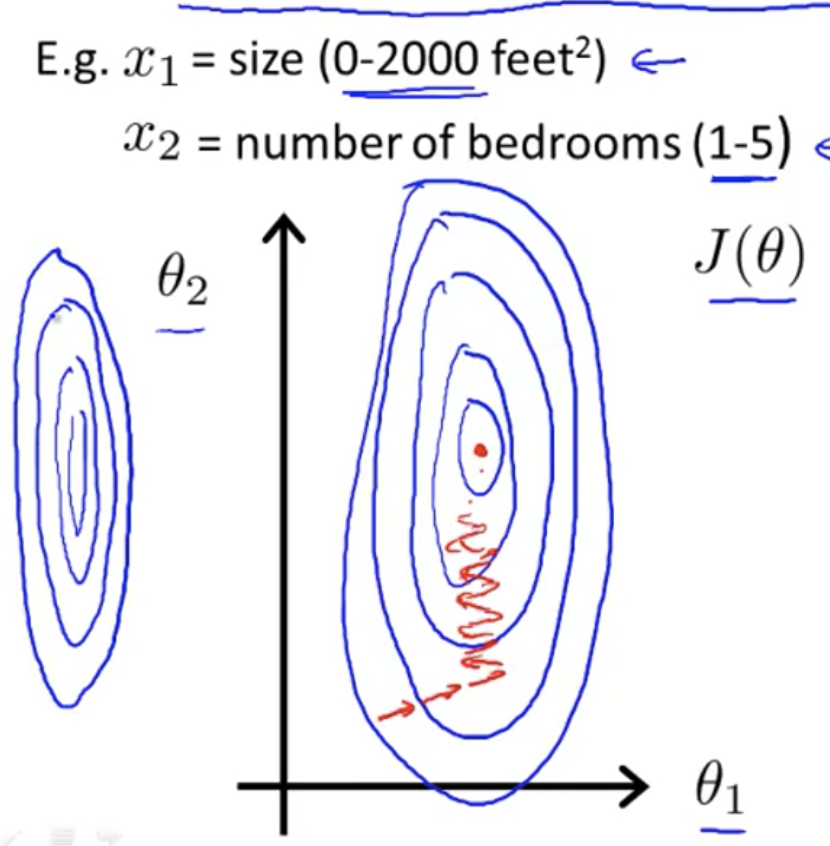
\includegraphics[scale=0.35]{椭圆.png}
\captionsetup{font={footnotesize}} 
\caption{随着$\theta$的变化$J$的变化}
\end{wrapfigure}

$$
\begin{aligned}
\mathbf{J(\mathbf{w})} &= \frac{1}{2m}\sum_{i=1}^{m}(\mathbf{\theta^T}x^{(i)}-y^{(i)})^2\\
&=\frac{1}{2m}\sum_{i=1}^mh_{\mathbf{\theta}}(\mathbf{x}^{(i)})-y^{(i)})^2
\end{aligned}
$$
其中,$m$是一次训练使用的数据的个数。
假如给定$\mathbf{J}$的数值,在$\theta_1,\theta_2\ldots,\theta_n$上画图,假如$n=2$将会得到一个椭圆。给定不同的$J$的数值,将会得到不同的椭圆,即等高线,如左图所示。

训练的过程所做的,就是初始化一个$\theta$并通过梯度下降的方法,使得$\theta$不断朝着最小值那里移动,让error更小。如左图红线所示。

\subsubsection*{特征缩放Feature Scaling}
椭圆的高矮胖瘦,取决于不同参数之间大小的比例,假如做一下特征缩放,就可以得到更加接近圆的图形。

训练的过程所做的,就是初始化一个$\theta$并通过梯度下降的方法,使得$\theta$不断朝着最小值那里移动,让error更小。如左图红线所示。

\subsubsection*{均值归一化:Mean normalization}

\section{统计学习初步}


\end{document}